\documentclass[aspectratio=169]{ISAE-Beamer}
\usefonttheme[onlymath]{serif}
\usepackage{amsmath,amssymb,amsthm}
\usepackage{bm}
\usepackage{arydshln,mathtools}
\usepackage{graphicx}
\usepackage{diffcoeff}
\usepackage{dsfont}
\usepackage{mathrsfs}
\usepackage{tcolorbox}

%\usepackage{multimedia}
\usepackage{media9}
\usepackage[backend=bibtex]{biblatex}

\graphicspath{{../Figures/},{./Figures/}}

\bibliography{bib_pHMSD}

\DeclareMathOperator{\Tr}{Tr}
\DeclareMathOperator*{\grad}{grad}
\DeclareMathOperator*{\Grad}{Grad}
\DeclareMathOperator*{\Div}{Div}
\renewcommand{\div}{\operatorname{div}}
\DeclareMathOperator*{\Hess}{Hess}

\DeclareMathOperator*{\argmax}{arg\,max}
\DeclareMathOperator*{\argmin}{arg\,min}

\newcommand{\crmat}[1]{\ensuremath{[#1]_{\times}}}

\def\onedot{$\mathsurround0pt\ldotp$}
\def\cddot{% two dots stacked vertically
	\mathbin{\vcenter{\baselineskip.67ex
			\hbox{\onedot}\hbox{\onedot}}%
}}

\renewcommand\bibfont{\scriptsize}


\makeatletter \renewcommand\d[1]{\ensuremath{%
		\;\mathrm{d}#1\@ifnextchar\d{\!}{}}}
\makeatother

\title[INFIDHEM meeting]{Port-Hamiltonian flexible multibody dynamics}

\institute[ISAE]
{\inst{1}ISAE-SUPAERO, Toulouse}

\author[Andrea Brugnoli]{Andrea Brugnoli}

\date[Munich, 24/03/20]{Tuesday, the 24th, 2020}

%\thanks{}

\begin{document}

\maketitle

\begin{frame}{Outline}

\tableofcontents

\end{frame}

\section{Previous work on multibody systems and the pH formalism}

\begin{frame}{Previous wok}

Using Lie Algebra and differential forms a pH model of a flexible link has already been proposed \footfullcite{macchelli_fl}. This model can be embedded in a complex multibody system\footfullcite{macchelli_flrig}. \\
\begin{overlayarea}{\textwidth}{0.55\textheight}
	\setlength{\abovedisplayskip}{1pt}
	\setlength{\belowdisplayskip}{1pt}
Advantages:
\begin{itemize}
	\item \onslide*<2->{Modular construction of flexible systems;}
	\item \onslide*<3->{Large deformations naturally considered.}
\end{itemize}
Drawbacks:
\begin{itemize}
	\item \onslide*<4->{Implementation really does not look trivial;}
	\item \onslide*<5->{Limited to one-dimensional systems;}
	\item \onslide*<6->{Numerical analysis not feasible;}
	\item \onslide*<7->{Model reduction techniques applicable.} 
\end{itemize}
\end{overlayarea}
\end{frame}

\section{PH formulation of a floating body}

\subsection{Floating frame formulation}

\begin{frame}{Floating frame based approach}
The floating frame approach relies on the hypothesis of small deformations: elastic motion is described w.r.t a reference that follows the large rigid motion\footfullcite{Noor_rev}. \\
\begin{overlayarea}{\textwidth}{0.5\textheight}
Advantages 
\begin{itemize}
	\item \onslide*<2->{The most used paradigm in multibody dynamics;}
	\item \onslide*<3->{For control applications most references adopt this approach;}
	\item \onslide*<4->{Model reduction techniques are applicable.} 
\end{itemize}
Drawbacks:
\begin{itemize}
	\item \onslide*<5->{Effect due to geometric non-linearities are not considered: not suitable for large deformations (substructuring can be employed to alleviate this).}
\end{itemize}
\end{overlayarea}
\end{frame}

\begin{frame}{Floating body kinematics}
\onslide*<1>{
\begin{tcolorbox}
	\begin{figure}[t]
		\centering
		\includegraphics[width=0.6\textwidth]{floating_body.eps} 
		\caption{Thin floating body undergoing a surface traction $\bm\tau$ and body force density $\bm\beta$}
		\label{fig:float_body}
	\end{figure}
\end{tcolorbox}
}
\onslide*<2>{
The velocity of a generic point is expressed by considering a small flexible displacement superimposed to the rigid motion
\[
\bm{v} = \bm{v}_P + \crmat{\bm{\omega}_P} (\bm{x}+\bm{u}_f) + \bm{v}_f.
\]
This equation is expressed in the body reference frame $\widehat{\bm{x}}, \widehat{\bm{y}}, \widehat{\bm{z}}$.  
\begin{itemize}
	\item $\bm{x}$ is the position vector of the current point;
	\item $\bm{v}_P,\, \bm{\omega}_P$ are the linear and angular velocities of point $P$;
	\item $\bm{v}_f := \dot{\bm{u}}_f$ is the time derivative of the deformation displacement $\bm{u}_f$ (computed in the body frame); 
	\item The cross map $\crmat{\bm{a}}$ denotes the skew-symmetric matrix associated to vector $\bm{a}$.
\end{itemize}

}
\end{frame}

\begin{frame}{Equations of motion}
The equations are obtained by application of the virtual work principle \footfullcite[Chapter 4]{simeon2013computational}. \\
\begin{overlayarea}{\textwidth}{0.8\textheight}
\only<1-2> {
	\begin{block}{Linear momentum balance}
		\setlength{\abovedisplayskip}{1pt}
		\setlength{\belowdisplayskip}{1pt}
		\only<1>{ 
		\begin{equation*}
		\begin{split}
		&m (\dot{\bm{v}}_P + \crmat{\bm{\omega}_P} \bm{v}_P) + \crmat{\bm{s}_u}^\top \dot{\bm{\omega}}_P  + \int_{\Omega} \rho \ddot{\bm{u}}_f \d{\Omega} = \\
		&\quad - \crmat{\bm{\omega}_P} \crmat{\bm{\omega}_P} \bm{s}_u - \int_{\Omega} 2 \rho \crmat{\bm{\omega}_P} \dot{\bm{u}}_f \d{\Omega} +  \int_{\Omega} \bm\beta \d{\Omega} + \int_{\partial \Omega} \bm\tau \d{\Gamma},
		\end{split}
		\end{equation*}
		}
		\only<2>{
			\begin{equation*}
			\begin{split}
			m\dot{\bm{v}}_P + \crmat{\bm{s}_u}^\top \dot{\bm{\omega}}_P +   \int_{\Omega} \rho \dot{\bm{v}}_f \d{\Omega}  = \\
			\textcolor{red}{\left[m \bm{v}_P + \crmat{\bm{s}_u}^\top \bm\omega_P +2 \int_{\Omega} \rho \bm{v}_f \d{\Omega} \right]_\times} \bm\omega_P +  \int_{\Omega} \bm\beta \d{\Omega} + \int_{\partial \Omega} \bm\tau \d{\Gamma}.
			\end{split}
			\end{equation*}
		}
	\end{block}

	\begin{itemize}
		\item $\rho$ is the mass density;
		\item $m = \int_{\Omega} \rho \d{\Omega}$ the total mass;
		\item  $\bm{s}_u = \int_{\Omega} \rho (\bm{x}+\bm{u}_f) \d{\Omega}$ the static moment.
	\end{itemize}
	}

\only<3-4> {
	\begin{block}{Angular momentum balance}
	\setlength{\abovedisplayskip}{1pt}
	\setlength{\belowdisplayskip}{1pt}
	\only<3>{
	\begin{equation*}
	\begin{split}
	\crmat{\bm{s}_u} (\dot{\bm{v}}_P + \crmat{\bm{\omega}_P} \bm{v}_P) + \bm{J}_u \dot{\bm\omega}_P + \int_{\Omega} \rho \crmat{\bm{x}+\bm{u}_f} \ddot{\bm{u}}_f \d{\Omega} + \crmat{\bm{\omega}_P} \bm{J}_u \bm{\omega}_P = \\ 
	- \int_{\Omega} 2\rho \crmat{\bm{x}+\bm{u}_f} \crmat{\bm\omega_P} \dot{\bm{u}}_f \d{\Omega} + \int_{\Omega}\crmat{\bm{x}+\bm{u}_f} \bm\beta \d{\Omega} + \int_{\partial \Omega}\crmat{\bm{x}+\bm{u}_f} \bm\tau \d{\Gamma}, \\
	\end{split}
	\end{equation*}
	}
	\only<4>{
		\begin{equation*}
		\begin{split}
		\crmat{\bm{s}_u} \dot{\bm{v}}_P  + \bm{J}_u \dot{\bm\omega}_P + \int_{\Omega} \rho \crmat{\bm{x}+\bm{u}_f} \dot{\bm{v}}_f \d{\Omega} = \\
		 \textcolor{red}{\left[\crmat{\bm{s}_u}^\top \bm\omega_P + 2 \int_{\Omega} \rho \bm{v}_f \d{\Omega} \right]_\times} \bm{v}_P +  \textcolor{red}{\left[\crmat{\bm{s}_u} \bm{v}_P + \bm{J}_u \bm\omega_P + 2 \int_{\Omega} \rho \crmat{\bm{x}+\bm{u}_f} {\bm{v}}_f \d{\Omega} \right]_\times} \bm\omega_P + 
		\\
		\int_{\Omega} \textcolor{red}{2 \left[\rho \bm{v}_P + \rho \crmat{\bm{x}+\bm{u}_f}^\top \, \bm\omega_P \right]_\times} \bm{v}_f \d{\Omega} + \int_{\Omega}\crmat{\bm{x}+\bm{u}_f} \bm\beta \d{\Omega} + \int_{\partial \Omega}\crmat{\bm{x}+\bm{u}_f} \bm{\tau} \d{\Gamma}.
		\end{split}
		\end{equation*}
	}	
	\end{block}
$\bm{J}_u:= \int_{\Omega} \rho \crmat{\bm{x}+\bm{u}_f}^\top\crmat{\bm{x}+\bm{u}_f} \d{\Omega}$ is the inertia matrix.
}
\only<5-6> {
	\begin{block}{Flexibility PDE}
		\setlength{\abovedisplayskip}{1pt}
		\setlength{\belowdisplayskip}{1pt}
	\only<5>{
	\begin{equation*}
	\begin{split}
	\rho (\dot{\bm{v}}_P + \crmat{\bm\omega_P} \bm{v}_P) + \rho (\crmat{\dot{\bm\omega}_P} + \crmat{\bm{\omega}_P}\crmat{\bm{\omega}_P})(\bm{x}+\bm{u}_f) + \rho (2 \crmat{\bm{\omega}_P} \dot{\bm{u}}_f + \ddot{\bm{u}}_f) = \\
	\Div{\bm\Sigma} + \bm\beta,
	\end{split}
	\end{equation*}
	}
	\only<6>{
	\begin{equation*}
	\begin{split}
	\rho \dot{\bm{v}}_P + \rho \crmat{\bm{x}+\bm{u}_f}^\top \dot{\bm\omega}_P  + \rho \dot{\bm{v}}_f = \\
	\textcolor{red}{\left[\rho \bm{v}_P + \rho \crmat{\bm{x}+\bm{u}_f}^\top \bm\omega_P + 2 \rho \bm{v}_f \right]_\times} \bm\omega_P + \Div{\bm\Sigma} + \bm\beta.
	\end{split}
	\end{equation*}
	}
	together with boundary conditions
	\begin{equation*}
	\begin{aligned}
	&\text{Neumann condition} \\
	&\text{Dirichlet condition} \\
	\end{aligned} \quad
	\begin{aligned}
	\bm\Sigma \cdot \bm{n}|_{\Gamma_N} &= \bm\tau|_{\Gamma_N}, \quad \text{$\bm{n}$ is the outward normal,} \\
	\bm{u}_f|_{\Gamma_D} &= \bm{\bar{u}}_f|_{\Gamma_D},
	\end{aligned}
	\end{equation*}
	\end{block}	
	
	\begin{itemize}
		\item $\bm\Sigma$ is the Cauchy stress tensor;
		\item The infinitesimal strain is given by $\bm\varepsilon  =  \Grad(\bm{u}_f) \quad \Grad = \frac{1}{2}[\nabla+\nabla^\top]$;
		\item To close the system,  Hooke's law $\bm\Sigma =  \bm{\mathcal{D}} \bm\varepsilon$, where $ \bm{\mathcal{D}}$ is the stiffness tensor.
	\end{itemize}
	}
\end{overlayarea}
\end{frame}


\subsection{Energies and momenta}

\begin{frame}{Energies and canonical momenta}
\begin{overlayarea}{\textwidth}{0.95\textheight}
Consider the total energy (Hamiltonian), given by the sum of kinetic and deformation energy:
\begin{equation*}
H = H_{\text{kin}} + H_{\text{def}}= \frac{1}{2} \int_{\Omega} \left\{\rho ||\bm{v}_P + \crmat{\bm{\omega}_P} (\bm{x}+\bm{u}_f) + {\bm{v}}_f||^2 + \bm\Sigma \cddot \bm\varepsilon \right\}  \d{\Omega}.
\end{equation*}

\only<1>{ 
	\begin{exampleblock}{Canonical momenta}
		\begin{equation*}
		\label{eq:momenta}
		\begin{aligned}
		\bm{p}_t &:= \diffp{H}{\bm{v}_P} = m \bm{v}_P + \crmat{\bm{s}_u}^\top \, \bm\omega_P + \int_{\Omega} \rho \bm{v}_f \d{\Omega}, \\
		\bm{p}_r &:= \diffp{H}{\bm\omega_P} = \crmat{\bm{s}_u} \bm{v}_P + \bm{J}_u \bm\omega_P + \int_{\Omega} \rho \crmat{\bm{x}+\bm{u}_f} \bm{v}_f \d{\Omega}, \\
		\bm{p}_f &:= \diffd{H}{\bm{v}_f} = \rho \bm{v}_P + \rho \crmat{\bm{x}+\bm{u}_f}^\top \, \bm\omega_P + \rho \bm{v}_f, \\
		\bm\varepsilon &:= \diffd{H}{\bm\Sigma} = \bm{\mathcal{D}}^{-1} \bm\Sigma,
		\end{aligned}
		\end{equation*}
	\end{exampleblock} 

}
\only<2>{
	\begin{exampleblock}{Canonical momenta}
	\setlength{\abovedisplayskip}{1pt}
	\setlength{\belowdisplayskip}{1pt}
	\begin{equation*}
	\begin{bmatrix}
	\bm{p}_t \\ \bm{p}_r \\ \bm{p}_f \\ \bm\varepsilon \\
	\end{bmatrix} = 
	\underbrace{\begin{bmatrix}
		m \bm{I}_{3\times 3} & \crmat{\bm{s}_u}^\top & \mathcal{I}_\rho^{\Omega} & 0 \\
		\crmat{\bm{s}_u} & \bm{J}_u & \bm{\mathcal{I}}_{\rho x}^{\Omega} & 0  \\
		(\mathcal{I}_\rho^{\Omega})^* & (\bm{\mathcal{I}}_{\rho x}^{\Omega})^* & \rho & 0  \\
		0 & 0 & 0 & \bm{\mathcal{D}}^{-1} \\
		\end{bmatrix}}_{\bm{\mathcal{M}}: \; \text{Mass operator}}
	\begin{bmatrix}
	\bm{v}_P \\ \bm{\omega}_P  \\ \bm{v}_f  \\ \bm\Sigma \\
	\end{bmatrix}, \qquad 
	\begin{aligned}
	\mathcal{I}_\rho^\Omega &:=\int_{\Omega} \rho (\cdot) \d{\Omega}, \\
	\bm{\mathcal{I}}_{\rho x}^{\Omega} &:= \int_\Omega \rho \crmat{\bm{x}+\bm{u}_f} (\cdot). \\
	\end{aligned}
	\end{equation*}	
	The mass operator $\bm{\mathcal{M}}$ is a self-adjoint, positive operator. It holds
	\begin{equation*}
	H_{\text{kin}} + H_{\text{def}} = \frac{1}{2} \langle \bm{e}_{\text{kd}}, \ \bm{\mathcal{M}} \bm{e}_{\text{kd}} \rangle, \qquad \bm{e}_{\text{kd}} = [\bm{v}_P; \, \bm{\omega}_P; \, \bm{v}_f; \bm{\Sigma}]
	\end{equation*}
\end{exampleblock} 
}
\only<3>{
Notice that the kinetic energy also depends on the flexible displacement
\[
\diffd{H_{\text{kin}}}{\bm{u}_f} = \crmat{\bm{p}_f} \bm{\omega_{P}}.
\]
This term is responsible for a coupling between the kinematic coordinates and the velocities.
}
\end{overlayarea}
\end{frame}

\subsection{PH formulation}

\begin{frame}{Generalized coordinates}
Generalized coordinates are required for a complete formulation:
\begin{itemize}
	\item $^i \bm{r}_P$ the position of point $P$ in the inertial frame of reference;
	\item $\bm{R}$ the direction cosine matrix (other attitude parametrizations are possible);
	\item $\bm{u}_f$ the flexible displacement;
\end{itemize}
The direction cosine matrix is converted into a vector by concatenating its rows
\begin{equation*}
\bm{R}_{\text{v}} = \text{vec}(\bm{R}^\top) = [\bm{R}_1 \; \bm{R}_2 \; \bm{R}_3]^\top,
\end{equation*}
where $\bm{R}_{1}, \bm{R}_{2}, \bm{R}_{3}$ are the rows of matrix $\bm{R}$. Furthermore the corresponding cross map will be given by
\begin{equation*}
\crmat{\bm{R}_{\text{v}}} = 
\begin{bmatrix}
\crmat{\bm{R}_1} \\
\crmat{\bm{R}_2} \\
\crmat{\bm{R}_3} \\
\end{bmatrix}, \qquad 
\crmat{\bm{R}_{\text{v}}} : \mathbb{R}^9 \rightarrow \mathbb{R}^{9 \times 3}.
\end{equation*}
\end{frame}

\begin{frame}{PH formulation}
The overall port-Hamiltonian formulation
\begin{equation*}
\setlength{\dashlinegap}{2pt}
\underbrace{
	{\left[ \begin{array}{c:c}
		\bm{I} & 0 \\
		\hdashline
		0 & \bm{\mathcal{M}} \\
		\end{array} \right]}
}_{\bm{\mathcal{E}}}
\diff{}{t}
\underbrace{\begin{bmatrix}
	^i \mathbf{r}_P \\ \bm{R}_{\text{v}} \\ \bm{u}_f \\\hdashline  \bm{v}_P \\ \bm\omega_P  \\ \bm{v}_f  \\ \bm\Sigma \\
	\end{bmatrix}}_{\bm{e}} = 
\underbrace{
	{\left[ \begin{array}{ccc:cccc}
		0 & 0 & 0 &  \bm{R} & 0 & 0 & 0 \\
		0 & 0 & 0 & 0 & \crmat{\bm{R}_{\text{v}}} & 0 & 0 \\
		0 & 0 & 0 & 0 & 0 & \bm{I}_{3\times 3} & 0  \\ 
		\hdashline
		-\bm{R}^\top & 0 & 0 & 0 & \crmat{\widetilde{\bm{p}}_t} & 0 & 0 \\
		0 & -\crmat{\bm{R}_{\text{v}}}^\top & 0 & \crmat{\widetilde{\bm{p}}_t} & \crmat{\widetilde{\bm{p}}_r} & \bm{\mathcal{I}}_{p_f}^\Omega & 0 \\
		0 & 0 & -\bm{I}_{3\times 3} & 0 & -(\bm{\mathcal{I}}_{p_f}^\Omega)^* & 0 & \Div \\
		0 & 0 & 0 & 0 & 0 & \Grad & 0 \\
		\end{array} \right]}
}_{\bm{\mathcal{J}}}
\underbrace{\begin{bmatrix}
	\partial_{\bm{r}_P}H \\ \partial_{\bm{R}_\text{v}}H \\ \delta_{\bm{u}_f} H \\\hdashline  \bm{v}_P \\ \bm\omega_P  \\ \bm{v}_f  \\ \bm\Sigma \\
	\end{bmatrix}}_{\bm{z}}.
\end{equation*} 
Variables $\widetilde{\bm{p}}_t, \widetilde{\bm{p}}_r$ are defined as: 
\[\widetilde{\bm{p}}_t = \bm{p}_t + \int_{\Omega} \rho \bm{v}_f \d{\Omega}, \qquad \widetilde{\bm{p}}_r = \bm{p}_r + \int_{\Omega} \rho \crmat{\bm{x} + \bm{u}_f}\bm{v}_f \d{\Omega}.\]
The operator $\bm{\mathcal{I}}_{p_f}^\Omega$ is defined as: $\bm{\mathcal{I}}_{p_f}^\Omega := \int_\Omega \left\{2 \crmat{\bm{p}_f} + \rho \crmat{\bm{v}_f} \right\}(\cdot) \d{\Omega}$.

\end{frame}

\begin{frame}{Floating body as a pHDAE system}
\begin{exampleblock}{Final pHDAE system}
	\setlength{\abovedisplayskip}{1pt}
	\setlength{\belowdisplayskip}{1pt}
This system fits into the framework detailed in \footfullcite{mehrmann2019structurepreserving} and extends it.
\begin{equation*}
\begin{aligned}
\bm{\mathcal{E}}(\bm{e}) \diffp{\bm{e}}{t} &= \bm{\mathcal{J}}(\bm{e}) \bm{z}(\bm{e}) + \bm{\mathcal{B}}_d(\bm{e}) \bm{u}_d + \bm{\mathcal{B}}_r(\bm{e}) \bm{u}_\partial, \qquad \text{where } \bm{u}_d:=\bm\beta \\
\bm{y}_d &= \bm{\mathcal{B}}_d^*(\bm{e}) \bm{z}(\bm{e}), \\
\bm{y}_r &= \bm{\mathcal{B}}_r^*(\bm{e}) \bm{z}(\bm{e}), \\
\bm{u}_\partial &= \bm{\mathcal{B}}_{\partial} \bm{z}(\bm{e}) =  \bm\Sigma \cdot \bm{n}|_{\partial \Omega} = \bm\tau|_{\partial \Omega}, \\
\bm{y}_\partial &= \bm{\mathcal{C}}_{\partial} \bm{z}(\bm{e}) = \bm{v}_f|_{\partial \Omega},
\end{aligned}
\end{equation*}
with $\bm{y}_r = (\bm{v}_P + \crmat{\bm{x}+\bm{u}_f}^\top \bm{\omega}_P)\vert_{\partial\Omega}, \; \bm{y}_d = (\bm{v}_P + \crmat{\bm{x}+\bm{u}_f}^\top \bm{\omega}_P + \bm{v}_f)\vert_{\Omega}$.
\end{exampleblock}
Operator $\bm{\mathcal{E}}$ is positive self-adjoint, $\bm{\mathcal{J}}$ is formally skew-symmetric.
The Hamiltonian  satisfies 
\begin{equation*}
\partial_{\bm{e}} H = \bm{\mathcal{E}}^* \bm{z}.
\end{equation*}
\end{frame}

\begin{frame}{Energy balance}
\onslide*<1-6>{
\begin{overlayarea}{\textwidth}{0.95\textheight}
State space $\mathscr{X} = \mathbb{R}^3 \times \mathbb{R}^9 \times \mathscr{L}^2(\Omega, \mathbb{R}^{3}) \times \mathbb{R}^3 \times \mathbb{R}^3 \times \mathscr{L}^2(\Omega, \mathbb{R}^{3}) \times \mathscr{L}^2(\Omega, \mathbb{R}^{3\times 3}_{\text{sym}}).$

\begin{equation*}
\begin{aligned}
\dot{H}(\bm{e}) &= \langle \partial_{\bm{e}} H, \partial_t {\bm{e}} \rangle_{\mathscr{X}},\\
\onslide*<2-6>{&= \langle \bm{\mathcal{E}}^* \bm{z}, \partial_t {\bm{e}} \rangle_{\mathscr{X}}, } \\
\onslide*<3-6>{&= \langle \bm{z}, \bm{\mathcal{E}} \partial_t {\bm{e}} \rangle_{\mathscr{X}}, \quad \text{Adjoint definition}, } \\
\onslide*<4-6>{&= \langle \bm{z}, \bm{\mathcal{J}}\bm{z} + \bm{\mathcal{B}}_d(\bm{e}) \bm{u}_d + \bm{\mathcal{B}}_r(\bm{e}) \bm{u}_\partial \rangle_{\mathscr{X}}, } \\
\onslide*<5-6>{&= \langle \bm{y}_\partial,  \bm{u}_\partial \rangle_{\mathscr{L}^2(\partial\Omega, \mathbb{R}^3)} + \langle \bm{\mathcal{B}}_d^* \bm{z}, \bm{u}_d \rangle_{\mathscr{X}} + \langle \bm{\mathcal{B}}_r^* \bm{z}, \bm{u}_\partial \rangle_{\mathscr{X}}, \quad \text{I.B.P. on } \bm{\mathcal{J}}, } \\
\onslide*<6>{&= \langle \bm{y}_\partial + \bm{y}_r,  \bm{u}_\partial \rangle_{\mathscr{L}^2(\partial\Omega, \mathbb{R}^3)} + \langle \bm{y}_d,  \bm{u}_d \rangle_{\mathscr{L}^2(\Omega, \mathbb{R}^3)}, } \\
\end{aligned}
\end{equation*}

\onslide*<5-6>{
where the integration by parts (Stokes theorem) has been used
\begin{equation*}
\setlength{\abovedisplayskip}{5pt}
\setlength{\belowdisplayskip}{5pt}
\int_{\Omega} \bm\Sigma \cddot \Grad(\bm{v}_f) \d{\Omega} + \int_{\Omega} \Div(\bm\Sigma) \cdot \bm{v}_f \d{\Omega} = \int_{\partial \Omega} (\bm\Sigma \cdot \bm{n}) \cdot \bm{v}_f \d{\Gamma} = \langle \bm{y}_\partial,  \bm{u}_\partial \rangle_{\mathscr{L}^2(\partial\Omega)}.
\end{equation*}}

\end{overlayarea}
}
\only<7->{\centering
\begin{exampleblock}{Power balance}
The power balance equals the power due to body force and surface traction
\begin{equation*}
\setlength{\abovedisplayskip}{5pt}
\setlength{\belowdisplayskip}{5pt}
\begin{aligned}
\dot{H}(\bm{e}) &= \int_{\partial \Omega} \bm\tau \cdot \bm{v} \d\Gamma + \int_{\Omega} \bm{\beta} \cdot \bm{v}  \d{\Omega},  \\
&= \int_{\partial \Omega} \bm{u}_d \cdot \bm{y}_d \d\Gamma + \int_{\Omega} \bm{u}_\partial \cdot (\bm{y}_\partial + \bm{y}_r)  \d{\Omega},
\end{aligned}
\end{equation*}
where $\bm{v} := \bm{v}_P + \crmat{\bm{\omega}_P} (\bm{x}+\bm{u}_f) + {\bm{v}}_f$ is the velocity field with the body
\end{exampleblock}

}

\end{frame}

\begin{frame}{Some remarks}

\begin{itemize}
	\item Generic linear elastic model can be included.
	\item Conservative forces are easily accounted for by introducing an appropriate potential energy. The gravitational potential
	\begin{equation*}
	H_{\text{pot}} = \int_{\Omega} \rho g \, ^i r_z \d{\Omega} = \int_{\Omega} \rho g \left[ ^i r_{P, z} +\bm{R}_z (\bm{x} + \bm{u}_f) \right] \d{\Omega}.
	\end{equation*}
	\item Geometric stiffening could be considered by adding a potential energy associated to centrifugal forces or using a substructuring technique.
	\item If case of vanishing deformations $\bm{u}_f \equiv 0$, the Newton-Euler equations on the Euclidean group $SE(3)$ are retrieved
	\begin{equation*}
	\begin{bmatrix}
	^i\dot{\bm{r}}_P \\ \bm{R}_{\text{v}} \\\dot{\bm{p}}_t \\ \dot{\bm{p}}_r \\
	\end{bmatrix} = 
	\begin{bmatrix}
	0 & 0 & \bm{R} & 0 \\
	0 & 0 & 0 & \crmat{\bm{R}_{\text{v}}} \\
	- \bm{R}^\top & 0 & 0 & \crmat{\bm{p}_t}\\
	0 & -\crmat{\bm{R}_{\text{v}}}^\top & \crmat{\bm{p}_t} & \crmat{\bm{p}_r} \\
	\end{bmatrix}
	\begin{bmatrix}
	\partial_{\bm{r}_P} H \\ \partial_{\bm{R}_{\text{v}}} H \\ \bm{v}_P \\ \bm{\omega}_P  \\
	\end{bmatrix}, \qquad
	\begin{bmatrix}
	\bm{p}_t \\ \bm{p}_r \\ 
	\end{bmatrix} = 
	\begin{bmatrix}
	m \bm{I} & \crmat{\bm{s}}^\top \\
	\crmat{\bm{s}} & \bm{J} \\
	\end{bmatrix}
	\begin{bmatrix}
	\bm{v}_P \\ \bm{\omega}_P  \\ 
	\end{bmatrix}.
	\end{equation*}
\end{itemize}
\end{frame}

\section{Discretization}

\begin{frame}{Partitioned finite element method}
	The procedure boils down to three simple steps
	\begin{enumerate}
		\item The system is written in weak form; 
		\item An integration by parts is applied to highlight the appropriate boundary control;
		\item A Galerkin method is employed to obtain a finite-dimensional system.
	\end{enumerate}
\end{frame}

\begin{frame}{Galerkin projection}
	Test functions $w$, state $e$ and effort functions $z$ are discretized using the same bases
	\[ \bm{w}(\bm{x}, t) = \bm{\phi}(\bm{x})^\top \mathbf{w}(t), \quad \bm{e}(\bm{x}, t) = \bm{\phi}(\bm{x})^\top \mathbf{e}(t), \quad \bm{z}(\bm{x}, t) = \bm{\phi}(\bm{x})^\top \mathbf{z}(t),
	\]
	\begin{exampleblock}{Finite-dimensional pHDAE system}
		\setlength{\abovedisplayskip}{3pt}
		\setlength{\belowdisplayskip}{3pt}
		After integration by parts of the $\Div$ operator
		\begin{equation*}
		\begin{aligned}
		\mathbf{E}(\mathbf{e}) \dot{\mathbf{e}} &= \mathbf{J}(\mathbf{e}) \mathbf{z}(\mathbf{e}) + \mathbf{B}_d(\mathbf{e}) \mathbf{u}_d + \mathbf{B}_\partial(\mathbf{e}) \mathbf{u}_\partial, \\
		\mathbf{y}_d &:= \mathbf{M}_d \widetilde{\mathbf{y}}_d = \mathbf{B}_d^\top \mathbf{z}(\mathbf{e}),  \\
		\mathbf{y}_\partial &:= \mathbf{M}_\partial \widetilde{\mathbf{y}}_\partial = \mathbf{B}_\partial^\top \mathbf{z}(\mathbf{e}).
		\end{aligned}
		\end{equation*}
	\end{exampleblock}
	
	\begin{block}{Dirichlet conditions}
		The set $\Gamma_D$ for the Dirichlet condition has to be non empty, otherwise the deformation field is allowed for rigid movement, leading to a singular mass matrix. Test and state shape functions must verify an homogeneous Dirichlet condition. 
	\end{block}
\end{frame}

\begin{frame}{Computation of the effort functions}
The computation of vector $\mathbf{z}$ is based on the discrete Hamiltonian  gradient:
\[
\diffp{H_d}{\mathbf{e}} = \mathbf{E}^\top \mathbf{z}, \qquad H_d = H_{d, \text{kin}}+H_{d, \text{def}}+H_{d, \text{pot}}.
\]
	The only term that requires additional care is $\bm{z}_{u}=\delta_{\bm{u}_f} H$.  \\
	Flexible displacement contribution to the power balance
	\[
	\dot{H}_u = \int_{\Omega} \diffp{\bm{u}_f}{t} \cdot \bm{z}_{u} \d{\Omega} = \int_{\Omega} \diffp{\bm{u}_f}{t} \cdot \diffd{H}{\bm{u}_f} \d{\Omega}
	\]
	Given that $\bm{u}_f = \bm{\phi}_u^\top \mathbf{u}_f, \; \bm{z}_u = \bm{\phi}_u^\top \mathbf{z}_u$, the discrete Hamiltonian rate assumes the expressions
	\begin{equation*}
	\dot{H}_{u, d}(\mathbf{u}_f) = 
	\begin{cases}
	\dot{\mathbf{u}}_f^\top \mathbf{M}_u \; \mathbf{z}_u, \\
	\displaystyle \dot{\mathbf{u}}_f^\top \diffp{H_d}{\mathbf{u}_f},
	\end{cases} \implies \mathbf{z}_u = \mathbf{M}_u^{-1} \diffp{H_d}{\mathbf{u}_f}, \quad \text{where } \mathbf{M}_u=\int_{\Omega} \bm{\phi}_u \, \bm{\phi}_u^\top \d{\Omega}
	\end{equation*}
	
\end{frame}

\section{Construction of multibody chain}

\subsection{General procedure for planar beams}
\begin{frame}{Thin planar beam case}
	\begin{columns}[T]
		\begin{column}{0.5\columnwidth}
				\begin{tcolorbox}
				\begin{figure}
					\centering
					\includegraphics[width=0.98\columnwidth]{beam.eps} 
					\caption{Floating beam.}
					\label{fig:beam}
				\end{figure}
			\end{tcolorbox}
		\end{column}
		\begin{column}{0.5\textwidth}
		\begin{block}{Beam discretized system}
			Neglecting the dependence on the deformation field in the mass matrix ($\mathbf{M}=\text{const}$)
			\begin{equation*}
			\begin{aligned}
			\mathbf{E} \dot{\mathbf{e}} &= \mathbf{J}(\mathbf{e}) \mathbf{z}(\mathbf{e}) + \mathbf{B} \mathbf{u}, \vspace{2mm} \\
			\mathbf{y} &= \mathbf{B}^{\top}  \mathbf{z}, \\
			\end{aligned}
			\end{equation*}
			with boundary variables
			\begin{equation*}
			\begin{aligned}
			\mathbf{u} &=  [F_{P}^x, \; F_{P}^y, \; T_{P}^z, \; F_{C}^x, \; F_{C}^y, \; T_{C}^z]^\top, \\
			\mathbf{y} &=  [v_{P}^x, \; v_{P}^y, \; \omega_{P}^z, \; v_{C}^x, \; v_{C}^y, \; \omega_{C}^z]^\top.
			\end{aligned}
			\end{equation*}
		\end{block}	
		\end{column}
	\end{columns}

\end{frame}

\begin{frame}{Revolute joint between beams}
\begin{columns}
	\begin{column}{0.5\textwidth}
		\begin{tcolorbox}
			\begin{figure}[t]
				\centering
				\includegraphics[width=0.9\columnwidth]{beam_int.eps} 
				\caption{Two hinged beams.}
				\label{fig:beam_int}
			\end{figure}
		\end{tcolorbox}
	\end{column}
	\begin{column}{0.5\textwidth}
	The interconnection variables are
	\begin{equation*}
	\begin{aligned}
	\mathbf{u}_1^{\text{int}} &= [F^x_{C_1}, \, F^y_{C_1}]^\top := \mathbf{F}_{C_1}, \\
	\mathbf{u}_2^{\text{int}} &= [F^x_{P_2}, \, F^y_{P_2}]^\top := \mathbf{F}_{P_2}, \\
	\mathbf{y}_1^{\text{int}} &= [v^x_{C_1}, \, v^y_{C_1}]^\top := \mathbf{v}_{C_1}, \\
	\mathbf{y}_2^{\text{int}} &= [v^x_{P_2}, \, v^y_{P_2}]^\top := \mathbf{v}_{P_2}.
	\end{aligned}
	\end{equation*}
	
	\end{column}
\end{columns}

\end{frame}

\begin{frame}{Final system}
\begin{block}{Hinged interconnected beams}
The transformer interconnection
\begin{equation*}
\mathbf{u}_1^{\text{int}} = -\mathbf{R}(\theta) \mathbf{u}_2^{\text{int}}, \qquad
\mathbf{y}_2^{\text{int}} = \mathbf{R}(\theta)^\top \mathbf{y}_1^{\text{int}},
\end{equation*}
where $\mathbf{R}(\theta)$ is the relative rotation matrix,	imposes the constraints on the velocity level and gives rise to a quasi-linear index 2 pHDAE.
\begin{equation*}
\begin{aligned}
\begin{bmatrix}
\mathbf{E}_1 & 0 & 0 \\ 
0 & \mathbf{E}_2 & 0 \\
0 & 0 & 0 \\
\end{bmatrix}
\begin{bmatrix}
\dot{\mathbf{e}}_1 \\ \dot{\mathbf{e}}_2 \\ \dot{\bm{\lambda}} \\
\end{bmatrix} &= 
\begin{bmatrix}
\mathbf{J}_1(\mathbf{e}_1) & 0 & -\mathbf{B}_1^{\text{int}} \mathbf{R} \\ 
0 & \mathbf{J}_2(\mathbf{e}_2) & \mathbf{B}_2^{\text{int}} \\
\mathbf{R}^\top \mathbf{B}_1^{\text{int} \top} & - \mathbf{B}_2^{\text{int} \top} & 0 \\
\end{bmatrix}
\begin{bmatrix}
\mathbf{z}_1  \\ 
\mathbf{z}_2  \\ 
\bm{\lambda} \\
\end{bmatrix}+ 
\begin{bmatrix}
\mathbf{B}_{\partial 1}^{\text{ext}} & 0 \\ 0 & \mathbf{B}_{\partial 2}^{\text{ext}} \\ 0 & 0 \\
\end{bmatrix} 
\begin{bmatrix}
\mathbf{u}_1^{\text{ext}} \\ 
\mathbf{u}_2^{\text{ext}} \\
\end{bmatrix}, \\
\begin{bmatrix}
\mathbf{y}_1^{\text{ext}} \\ \mathbf{y}_2^{\text{ext}} \\
\end{bmatrix}  &= \begin{bmatrix}
\mathbf{B}_{\partial 1}^{\text{ext} \top} & 0 & 0 \\
0 & \mathbf{B}_{\partial 2}^{\text{ext} \top} & 0 \\
\end{bmatrix} \begin{bmatrix}
\mathbf{z}_1  \\ 
\mathbf{z}_2  \\ 
\bm{\lambda} \\
\end{bmatrix}.
\end{aligned}
\end{equation*}
\end{block}
\end{frame}

\begin{frame}{Equivalence of gyrator and transformer interconnection}
The same result can be obtained by using a pHDAE system and a gyrator interconnection.  It is sufficient to interchange the role of output and input of the second system $\mathbf{u}_2^{\text{int}} \leftrightarrow \mathbf{y}_2^{\text{int}}$. 
\begin{figure}[t]
	\centering
	\includegraphics[width=0.46\textwidth]{block_hinged_beam.eps} \hspace{.5cm}
	\includegraphics[width=0.46\textwidth]{block_hinged_beam_DAE.eps} 	
\end{figure}

\end{frame}

\subsection{The linear case}

\begin{frame}{Linear case}
	Hypothesis:
	\begin{enumerate}
		\item small angular velocities;
		\item small relative configuration.
	\end{enumerate} 
	
	\begin{equation*}
	\label{eq:mbd_linear}
	\begin{bmatrix}
	\mathbf{M}_{rr} & \mathbf{M}_{rf} & 0 \\ 
	\mathbf{M}_{fr} & \mathbf{M}_{ff} & 0 \\
	0 & 0 & 0 \\
	\end{bmatrix}
	\begin{bmatrix}
	\dot{\mathbf{p}}_r \\ \dot{\mathbf{p}}_f \\ \dot{\bm{\lambda}} \\ 
	\end{bmatrix} = 
	\begin{bmatrix}
	0 & 0 & \mathbf{G}_r^\top \\ 
	0 & \mathbf{J}_{ff} & \mathbf{G}_f^\top \\ 
	-\mathbf{G}_r & -\mathbf{G}_f & 0 \\
	\end{bmatrix}
	\begin{bmatrix}
	\mathbf{p}_r \\ \mathbf{p}_f \\ {\bm{\lambda}} \\ 
	\end{bmatrix} + 
	\begin{bmatrix}
	\mathbf{B}_r \\ \mathbf{B}_f \\ 0 \\
	\end{bmatrix}\mathbf{u}.
	\end{equation*}
	with Hamiltonian $H = \frac{1}{2} \mathbf{p}^\top\mathbf{M}\mathbf{p}$. The modular construction of complex multi-body systems is then analogous to a sub-structuring technique \footfullcite{substructuring}.  
\end{frame}

\begin{frame}{Model and index reduction}
\only<1>{
\begin{block}{Model reduction}
Such system can be reduced using Linear model reduction methods directly in the DAE\footfullcite{phdae_red}. Vector $\mathbf{p}_f$ is projected on a meaningful subspace $\mathbf{p}_f \approx \mathbf{V}_f^{\text{red}} \mathbf{p}_f^{\text{red}}$
\begin{equation*}
\begin{bmatrix}
\mathbf{M}_{rr} & \mathbf{M}_{rf}^{\text{red}} & 0 \\ 
\mathbf{M}_{fr}^{\text{red}} & \mathbf{M}_{ff}^{\text{red}} & 0 \\
0 & 0 & 0 \\
\end{bmatrix}
\begin{bmatrix}
\dot{\mathbf{p}}_r \\ \dot{\mathbf{p}}_f^{\text{red}} \\ \dot{\mathbf{\lambda}} \\ 
\end{bmatrix} = 
\begin{bmatrix}
0 & 0 & \mathbf{G}_r^\top \\ 
0 & \mathbf{J}_{ff}^{\text{red}} & \mathbf{G}_f^{\text{red} \top} \\ 
-\mathbf{G}_r & -\mathbf{G}_f^{\text{red}} & 0 \\
\end{bmatrix}
\begin{bmatrix}
\mathbf{p}_r \\ \mathbf{p}_f^{\text{red}} \\ {\mathbf{\lambda}} \\ 
\end{bmatrix} + 
\begin{bmatrix}
\mathbf{B}_r \\ \mathbf{B}_f^{\text{red}} \\ 0 \\
\end{bmatrix}\mathbf{u},
\end{equation*}
\end{block}
}

\only<2>{
\begin{block}{Index reduction}
\begin{equation*}
\begin{aligned}
\mathbf{M} \dot{\mathbf{p}} &=  \mathbf{J}\mathbf{p} + \mathbf{G}^\top \bm{\lambda} + \mathbf{B}\mathbf{u}, \\ 
\mathbf{0} &= \mathbf{G}\mathbf{p},
\end{aligned}
\end{equation*}
A null space matrix can employed to eliminate the Lagrange multiplier and preserve the port-Hamiltonian structure. 
\[
\mathrm{range}\{\mathbf{P}\} = \mathrm{null}\{\mathbf{G}\}.
\]
Then, the range of $\mathbf{P}$ automatically satisfies the constraints. Considering the transformation $\widehat{\mathbf{p}} = \mathbf{P} \mathbf{p}$ and pre-multiplying the system by $\mathbf{P}^\top$ an equivalent ODE is obtained
\[
\widehat{\mathbf{M}} \ \dot{\widehat{\mathbf{p}}} =  \widehat{\mathbf{J}} \ \widehat{\mathbf{p}} + \widehat{\mathbf{B}} \ \mathbf{u},
\]
with $\widehat{\mathbf{M}} = \mathbf{P}^\top \mathbf{M} \mathbf{P}, \; \widehat{\mathbf{J}} = \mathbf{P}^\top \mathbf{J} \mathbf{P}, \; \widehat{\mathbf{B}} = \mathbf{P}^\top \mathbf{B}$.
\end{block}
}

\end{frame}

\begin{frame}{Conclusion}
Summarizing:
	\begin{itemize}
		\item port-Hamiltonian formulation of floating bodies;
		\item finite element discretization;
		\item interconnection of subcomponents;
		\item linearized case.
	\end{itemize}
Some open questions
\begin{itemize}
	\item stability and convergence of finite element;
	\item time discretization;
	\item non-linear model reduction od pHDAE;
	\item control strategies.
\end{itemize}
\centering
\Large Additional information \url{https://arxiv.org/abs/2002.12816} \\
\end{frame}


\begin{frame}{}
\centering

\Huge Thanks for your attention \\
\Huge Questions?
\end{frame}

\begin{frame}[allowframebreaks]{References}
\printbibliography
%\nocite{*}
\end{frame}

\end{document}
